\item A montagem consiste de duas barras de \SI{4}{\kilogram} que estão conectadas por pinos aos dois discos de \SI{5}{\kilogram}.
Se as barras são liberadas do repouso quando $\theta=\SI{60}{^{\circ}}$, determine suas velocidades angulares no instante $\theta=\SI{30}{^{\circ}}$. Suponha que os discos rolam sem deslizar.

\import{../answers}{answer-15}

\begin{flushright}
	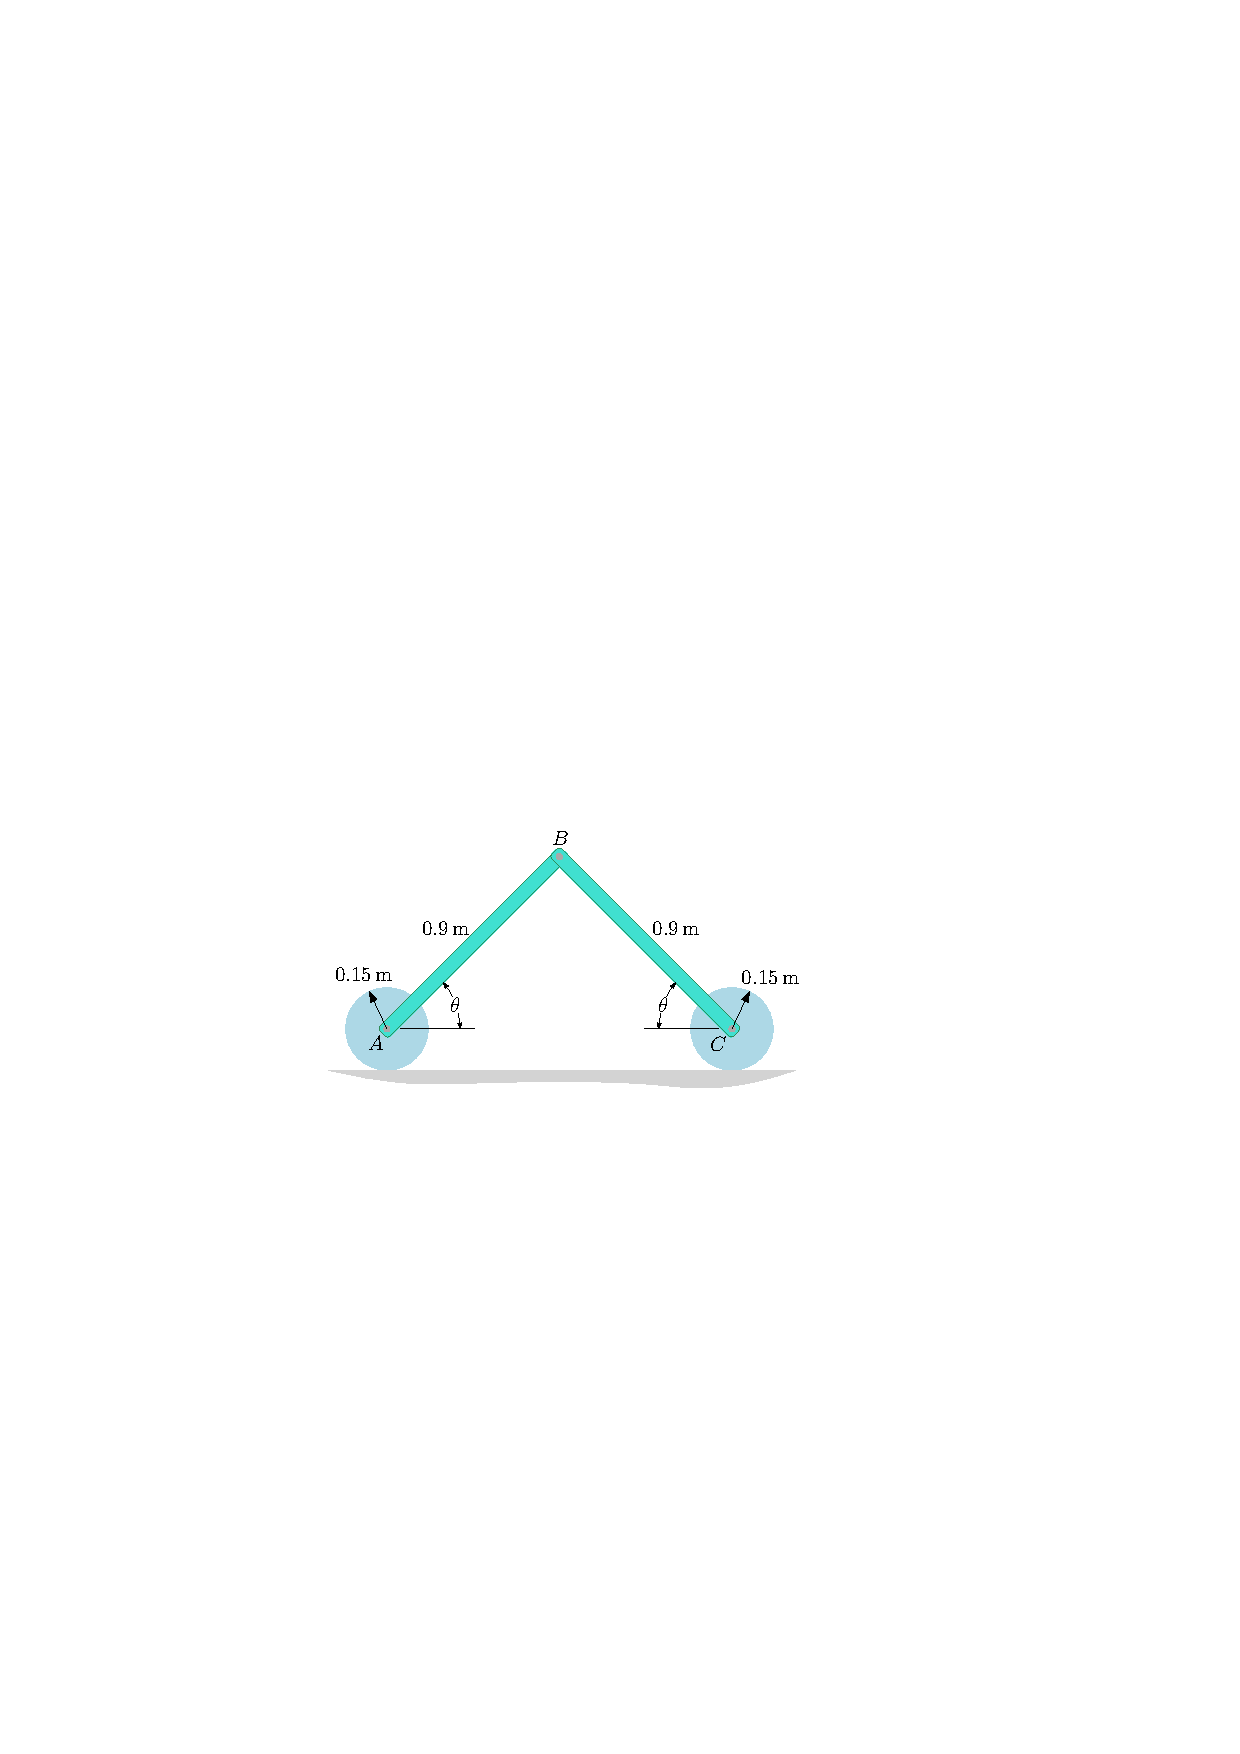
\includegraphics[scale=1.2]{../../images/draw_7}
\end{flushright}